\chapter{Hyperledger Fabric}
\label{ch:fabric}
Fabric\cite{androulaki2018hyperledger} is an open-source permissioned blockchain. It is designed for enterprises; therefore, it has a modular design to support multiple use cases of industry. It is the first blockchain to allow plug-able consensus protocol in ordering service, So users can choose and plug consensus according to threat model and application. It is first blockchain to allow developers to write smart contracts/ applications in general-purpose programming languages like Go, Java, etc., which makes developing application fast, easy and cost-efficient as no special training is required for the domain-specific languages to write smart contracts. Fabric also allows plug-able identity management system, so that enterprises can plug and use industry-standard identity management systems. Fabric introduces a new blockchain paradigm and changes the way blockchains handle the current problems in blockchains, such as performance attacks, non-determinism, and resource exhaustion. 
 
\section{Architecture}
Fabric replaces the old standard order-execute blockchain architecture and introduces the novel execute-order-validate blockchain architecture. This new paradigm eliminates the need for every peer to execute every transaction sequentially as in order-execute design, thus increase the effective performance and throughput. A Fabric application has two parts.
\begin{itemize}
    \item \textbf{Chaincode:} A smart contract, called \textit{chaincode}, is a program code that implements the application logic and runs during the execution phase.
    \item \textbf{Endorsement:} \textit{endorsement} policy contains a list of endorsers for a transaction of a chaincode, and this list is used in the validation phase to validate the transaction. 
    % A normal user can not change endorsement policy; you need special permission to change it.
    
\end{itemize}
\clearpage

A fabric network is made up of various types of nodes taking up one of these three roles.:


\begin{itemize}
    \item \textbf{Client:} The client represents the entity that acts on behalf of an end-user. Client is the initiator of the transaction; firstly, it submits transaction proposals for execution to the endorser peers for endorsement and, finally, it sends the transaction along with endorsements to the orderer peers of ordering.  
    \item \textbf{Peers:} Peers are of two types, normal peer and endorser peers.
    All peers have the responsibility of maintaining ledger by validating the transaction, appending new blocks to ledger, and update ledger state by updating \textit{key-value} pairs, whereas endorser peers also have an added responsibility of endorsing transaction by executing chaincode function given in transaction and returning the result to the client. Endorsers for a chaincode are mentioned in the endorsement policy.
    
    \item \textbf{Ordering Service Nodes (OSN):} These nodes are also known as Orderers. In short, the work of the ordering service is to establish the total order of all transactions. Orderers have no role in the application state and are unaware of it and do not participate in any phase of the transaction except ordering. This independence from the application and other peers allows consensus in Fabric to plug-able and consensus protocol can be chosen as per the need of the application and  trust model. 
\end{itemize}
\subsection{Transaction Flow}
\begin{figure}[!h]
    \centering
    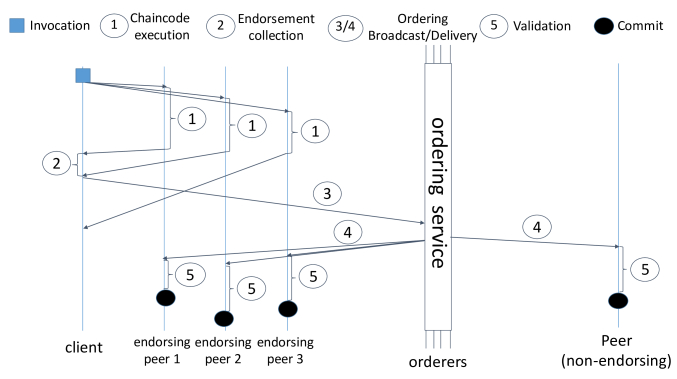
\includegraphics[scale=0.6]{images/fabrictxn.jpeg}
    \caption{Fabric Transaction Flow \cite{androulaki2018hyperledger}}
    \label{fig:fabrictxn}
\end{figure}
\begin{enumerate}
    \item Client creates a proposal for a transaction and sends it to the endorser peers mentioned in endorsement policy and wait for endorsements.
    \item Upon receiving the proposal for transaction endorser peers execute the transaction and send back the result to the client as endorsement. This phase is called \textit{execute} phase.
    \item Upon getting enough endorsements to full fill the endorsement policy, client groups the endorsements, create a transaction, and submit it to the ordering service.
    \item Upon receiving transaction, orderers run consensus protocol, output a total ordered sequence of endorsed transaction, and create a block of these ordered transaction. These blocks are then broadcasted to all the peers, either directly or via gossip. This phase is called \textit{order} phase.
    \item Upon receiving blocks, peers validate all the transactions in the block and mark invalid transaction and append this block to their local ledgers. This phase is called \textit{validate} phase.
    \item After block is appended to the ledger the transaction is commited to the blockchain ledger.
\end{enumerate}

Now we will see each phase in detail.

\subsection{Execution Phase}
\label{ssec:exec}
In this phase, Client sends its proposal for the transaction to the endorser peers for execution. A proposal contains the client's identity, a nonce for the client, i.e., one-time-use random number, transaction-id and transaction's payload(parameters, an operation, and chaincode ID).

 The endorsers execute the proposed operation on the chaincode. As a result of the execution, each endorser produces a value \textit{writeset} and \textit{readset}, writeset consists of the key-value pairs that are to be updated, and readset consists of keys with their version number that are read during execution. After the execution, the endorsement is sent back to the client, containing an endorser ID, writeset, readset, transaction ID, and endorser signature. The client waits for enough endorsements to satisfy the endorsement policy. Moreover, all endorsements should have the same execution result. If all endorsements have the same result and we have enough endorsements then client makes a transaction and sends it to ordering service.
\subsection{Ordering Phase}
Once client has created a transaction, it submits the transaction for next phase i.e., Ordering phase.
    The ordering service establishes a consensus on the total order of the transactions submitted to a channel. Moreover, The ordering service bundles multiple transactions into blocks and then delivers them to all peers. An orderering service can support multiple blockchains.

The ordering service offers two APIs. 
\begin{itemize}
    \item \textbf{broadcast(txn):} Broadcast is used by Client to send the transaction \textit{txn}  to all the orderer nodes in the channel.
    \item \textbf{deliver(s):} This function delivers the block with sequence number \textit{s} in the legder.
    
\end{itemize}

The ordering service in Fabric is as an independent service and it has no role in validation phase, executions phase, and does not maintain any state.
\subsection{Validation Phase}
Upon receiving a block, peers validate the transaction by following the below steps sequentially:
\begin{enumerate}
\item \textbf{Endorsement Policy Evaluation:} In this step, peer validates all the transactions whether they full fill the endorsement policy or not. As the evaluation is independent for all the transactions this is done in parallel for all transactions. Transactions unable to full fill the endorsement policy, are marked invalid.
\item \textbf{Read-Write Conflict Check:} This step validates transaction's readset and writeset versions. This evaluation is dependent on the ledger state, So this check is performed sequentially on all the transactions in the block. Transactions are marked invalid, if they fail the check. 
\item \textbf{Ledger Update Phase:} This the final step in the validation phase. Peers append the block to their local ledger.
If any of the check fails, that is also reflected here in the form of bitmask. Invalid transactions are also included in the block, in-order to keep track or it may be helpful in certain scenarios.
\end{enumerate}


\section{Fabric Network}

In this section, We will discuss the network components of a Fabric network and its setup.

A Fabric network\cite{fabric_network} is an infrastructure that provides blockchain services. Mostly, multiple stakeholders are interested in having a ledger application they can trust. So they work together and form a fabric network. All the policies are agreed and set by the stakeholders together.
 
\begin{figure}[!h]
    \centering
    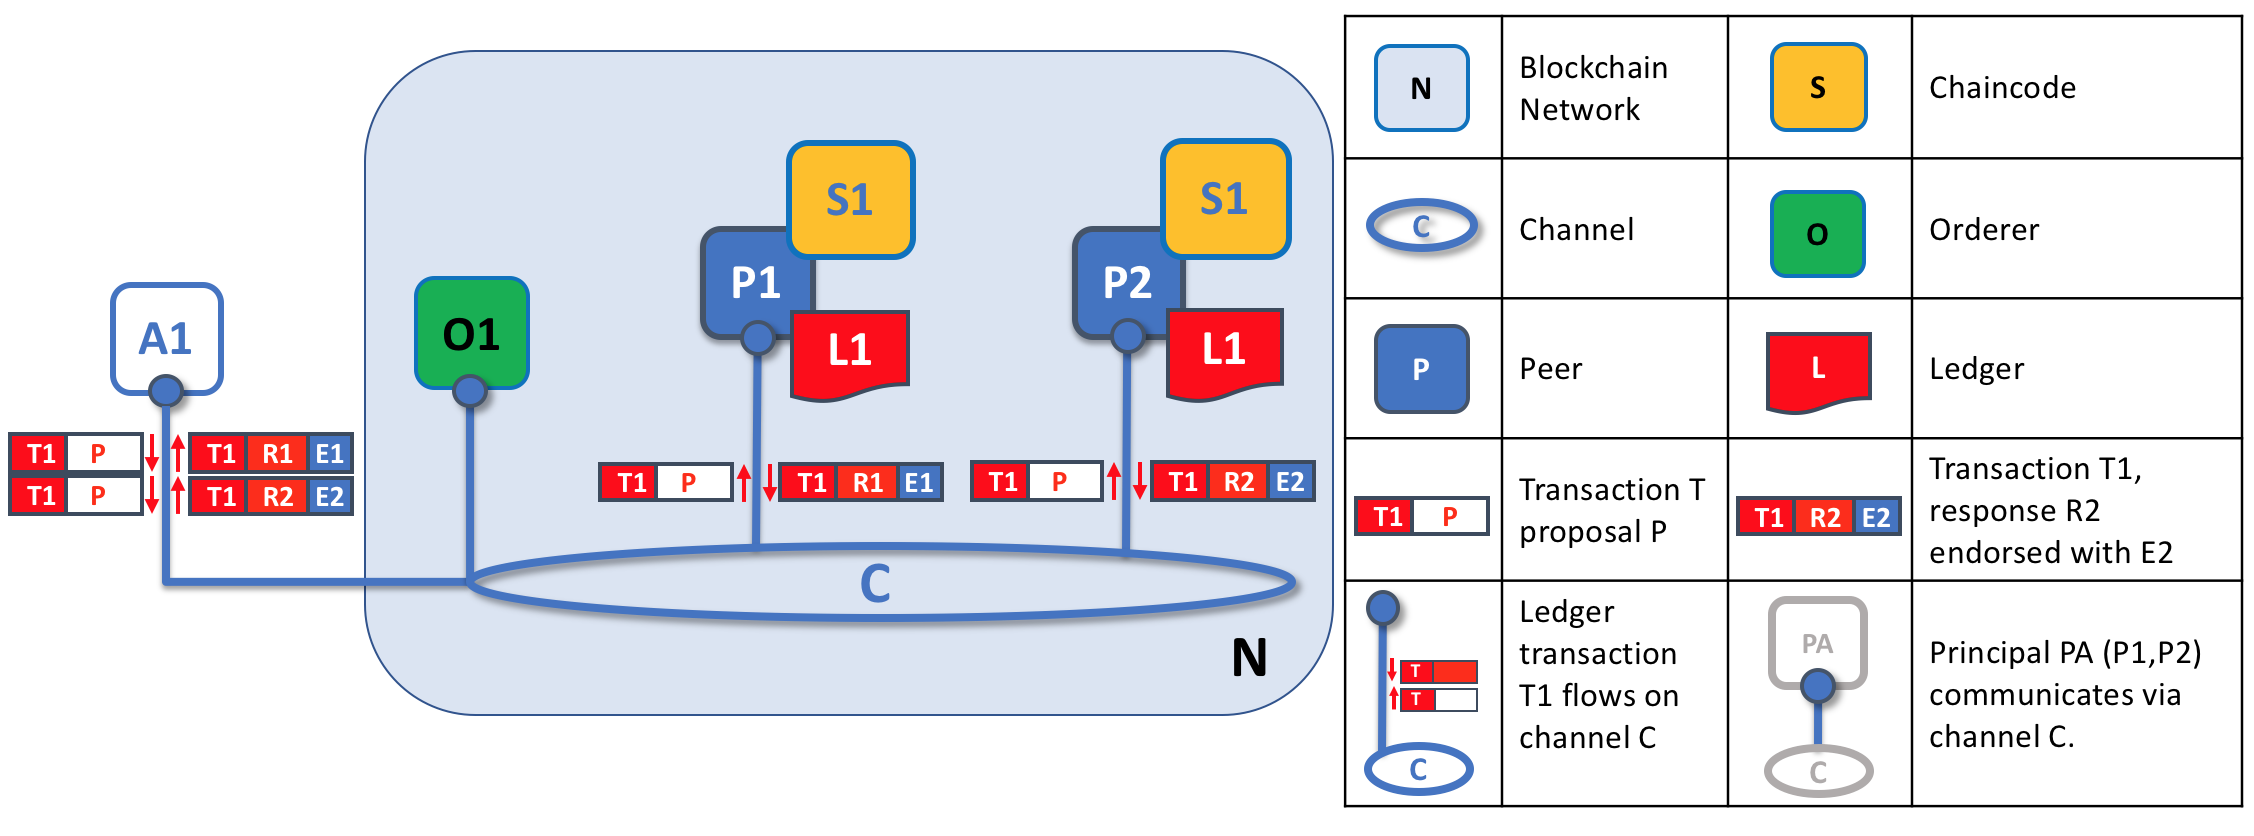
\includegraphics[width=1\textwidth]{images/fabric_network.png}
    \caption{Example of fabric network  \cite{fabric_network_image}}
    \label{fig:fabric_network}
\end{figure}
\subsection{Components of a Network\cite{fabric_glossary}}
\begin{enumerate}
    \item \textbf{Ledgers:\label{subsub:ledger}}
    
     Fabric \textit{ledger} consists of two parts:
     \begin{itemize}
         \item Blockchain : Blockchain is a normal immutable append-only chain of blocks.
         \item Database : Database or World state contains set key-value pairs added, deleted, or updated by validated and committed transactions. 
     \end{itemize}.  

\item \textbf{Smart contract(s) (aka chaincode):}
Smart contract is also know as \textit{chaincode} in Fabric. It is responsible for managing access and state of the blockchain. Chaincode is installed on peer nodes and used via a channel to which it is instantiated.


\item \textbf{Peer nodes:}
Peer nodes are an important member of the network. Peer nodes maintain a ledger by running the installed chaincode which updates state of ledger. A Peer can host multiple ledgers and chaincodes. A Network can have multiple peer nodes. A peer can also be an \textit{endorser}.
\item \textbf{Ordering service:}
The job of ordering service is to order the transactions and make blocks. The transactions are ordered on first-come-first-serve basis for all channels. Ordering service is cluster of orderers.
\item \textbf{Channel:}
\textit{channel} is a way to create  private “subnet” of network members, for data isolation and confidentiality, it ensures privacy from other channels. Every channel has its own ledger maintain by all the peers in that channel.

\item \textbf{Fabric Certificate Authorities:}
Fabric Certificate Authorities is a default certificate authority. It creates and validates the identities of the members of the network and users.
\end{enumerate}

\subsection{Network Setup }
In this section, we discuss how to setup a sample fabric  network using fabric-samples BYFN (i.e. Build Your First Network) example \cite{byfn}\cite{medium_byfn}.
\subsubsection{Pre-requisites}
\begin{enumerate}
    \item \textbf{Install}: You can follow the steps given \href{https://hyperledger-fabric.readthedocs.io/en/release-2.0/prereqs.html}{\textit{here}.}
    \begin{itemize}
    \item docker
    \item docker-compose
    \item golang
    \end{itemize}
    \item \textbf{Clone repository}: Download the fabric-samples repository from \href{https://github.com/hyperledger/fabric-samples}{here}
    \begin{itemize}
        \item \begin{lstlisting}[language=bash]
  $ git clone https://github.com/hyperledger/fabric-samples.git
\end{lstlisting}
\end{itemize}
\item \textbf{Download:} platform specific binaries and docker images
\begin{itemize}
    \item docker images
    \begin{itemize}
         \item fabric-orderer
        \item fabric-peer
        \item fabric-tools
        \item fabric-ca
        \item fabric-ccenv
    \end{itemize}
      \item platform specific binaries
    \begin{itemize}
        \item fabric-ca-client
        \item fabric-ca-server
        \item idemixgen
        \item congiftxlator
        \item discover
        \item cryptogen
        \item peer
        \item orderer
        \item configtxgen
    \end{itemize}
    \item The above mentioned docker images and platform specific binaries can be downloaded using below command \begin{lstlisting}[language=bash]
   curl -sSL https://bit.ly/2ysbOFE | bash -s \
           -- <fabric_version> <fabric-ca_version> <images_version>
\end{lstlisting} 

\end{itemize}
\end{enumerate}

\begin{figure}[!h]
    \centering
    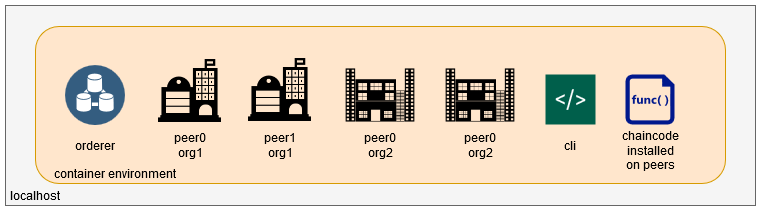
\includegraphics[scale=0.55]{images/byfn.png}
    \caption{BYFN - docker images\cite{medium_byfn}}
    \label{fig:fabric_network}
\end{figure}

After installing and downloading all the prerequisites we can now run the Fabric network. First navigate to "\textit{fabric-samples/first-network}".
There we  find two config files, "\textit{configtx.yaml}" and "\textit{crypto-config.yaml}". We can update these configuration files to build the fabric network according to our needs.



There is also a script "byfn.sh" in \textit{first-network} which manages the network. Fabric network for \textit{first-network} is shown in the Figure \ref{fig:fabric_network} . The script supports the following options:
\begin{itemize}
    \item \textbf{generate: } Generates required certificates and genesis block for the network using  \textit{configtxgen} binary.
    \item \textbf{up: } Up generates crypto material first, then brings the network up using docker-compose and run a sample application to test the network.
     \item \textbf{down: } Tears down the network by stopping and removing all docker images and deletes  crypto material.
    
\end{itemize}